\Chapter{Minták generálása}

\begin{comment}{Az alkalmazandó módszernél majd érdemes jobban részletezni, hogy ANN-el fog történni.}
\end{comment}

\section{Tanító mintapontok előállítása}

A megvalósító neurális hálózat betanítása felügyelt tanulás módszerrel történik. A minták alapján történő tanulás lényege, hogy az eljárás során a be- és kimeneti mintapárokból igyekszünk megfelelő ismereteket kinyerni és ezzel a rendszer viselkedését módosítani. A hálózat feladata, hogy megtanulja a rendelkezésre álló mintapont párok által reprezentált bemenet-kimenet leképezést. Ehhez elő kell állítani a megfelelő adathalmazt.

Az adathalmaz előállítása elött definiálni kell a rajzolás dinamikáját. A vonal kirajzolás sorrendje mellet fontos a vonal vastagsága is. Az kézírás ugyan sokat változott, de az alapjai megmaradtak. A stroke-ok vastagsága az ecset gyorsaságától, az ecsetre ható nyomás nagyságától függ. A megfelelően rajzolt vonalakat nagyon fontosnak tartják a kínaiak, mivel a kultúrájukhoz tartozik. A kalligráfia elárulhatja az ember nemét, korát, személyességét. Kézzel írott karakterekre láthatunk néhány példát \aref{fig:calligraph}. ábrán.

\begin{figure}
\centering
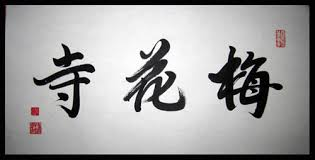
\includegraphics[scale=0.8]{calligraphy}
\caption{Példa néhány kézzel írott kínai karakterre}
\label{fig:calligraphy}
\end{figure}

\subsection{Vonal vastagság}

A következőkben részletezném a vonal vastagság változását a stroke-ok rajzolásának függvényébe. 

\begin{itemize}
\item A stroke-ok vége elvékonyul, ezt a valóságban az ecset hirtelen felemelésével érik el. (Van néhány kivétel, mint például a \textit{right fally} 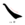
\includegraphics[scale=1.0]{right_fally}) 
\item Ha egy stroke végéből kezdődik egy másik stroke, akkor azok találkozásánál a vonalvastagság növekszik.
\item A horizontális vonalak közepe elvékonyul majd a végén újra vastagabb lesz. A vastagságot súlyokkal könnyedén lehet definiálni.

\begin{center}
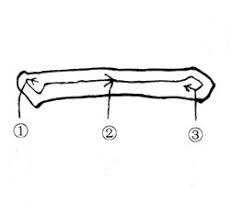
\includegraphics[scale=0.6]{horizontal_line}
\end{center}

\item A kampós vonalaknál (hooked stroke) a "kampó" hirtelen vékonyodással és irányváltoztatással jár. Az ecset hirtelen felemelésével érik el. Általában a kampó 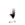
\includegraphics[scale=1.0]{hook} stroke része.
\item A további stroke-ok általában állandó vonal vastagsággal (ecset gyorsaság állandó). A kézzel írás és festés egyén függő.
\end{itemize}

\subsection{Környezet a karakterek kirajzolásához}

\begin{itemize}
\item A kínai karakterek festése papíron történik. A mi esetünkben ez a képernyő. A karakterek fekete-fehér színüek. A szürke árnyalatokat $[0, 255]$ intervallumon vett egész értékek reprezentálják. Az ideálisan kirajzolt karakter fekete-fehér színű, és ahhoz a generálás során adhatunk hozzá szürke pixelek formájában zajt.

A karakterek rajzolásához a Python programozási nyelv és a hozzá elérhető eszközök tüntek megfelelőnek. Egy $512 \times 512$ pixelből álló fehér kép kirajzolása az alábbi módon történik a segítségével.
\begin{python}
img = np.zeros((512, 512, 3), np.uint8)
img[0:512] = (255, 255, 255)
\end{python}

\item A festés alapvető eszköze az ecset. Az ecset lenyomássa egy ellipszis alakot hozz létre. A festés során az ecset elfordul (megfigyelésünk szerint 45fokban). Az ellipszis területe megnő, ha a festés gyorsasága csökken, ellenkező esetben csökken. Az ellipszist könnyedén lehet rajzolni az OpenCV \texttt{ellipse} függvénye segítségével, amelynek a paraméterezése a következő.
\begin{python}
cv2.ellipse(img, center, axes, angle, start_angle, 
	end_angle, color, thickness=1, lineType=8, shift=0) 
\end{python}
\end{itemize}

\subsection{Karakterek kirajzolása}

\begin{enumerate}
\item Poligonos közelítés: A kínai karakter ebben az esetben pontok halmaza és az ezeket összekötő poligonok. Minél több ponttal definiáljuk a karaktert annál jobb minőségű képet érünk el, viszont a számítás igényünk növekszik.
\item Procedurális rajzolás: Ellipsziseket rajzolunk a képernyőre a kínai karakternek megfelelően. Az ellipsziseket érintő egyenesekkel összekötjük. Az ellipszisek tengelyeinek mérete különbözhetnek egymástól.
\begin{center}
\begin{tabular}{ c c }
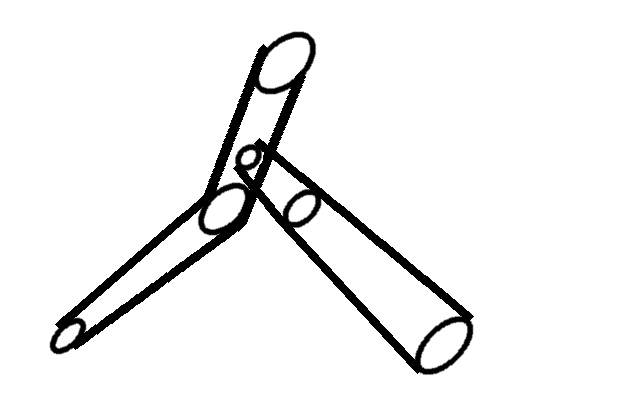
\includegraphics[scale=0.25]{proc_draw1} & 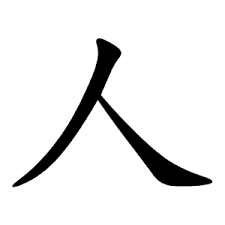
\includegraphics[scale=0.5]{ren}
\end{tabular}
\end{center}
Az ellipszisek koordinátáit egy-egy 5 dimenziós vektorral adhatjuk meg
\begin{align*}
P_1 &= (x_1, y_1, d_{x_1}, d_{y_1}, s_1) \\
P_2 &= (x_2, y_2, d_{x_2}, d_{y_2}, s_2).
\end{align*}
Az 'x' és 'y' koordináta párral az ellipszis középpontját adjuk meg. A $d_x$ és $d_y$ az ellipszis irányvektorai, amit majd a görbe kirajzolásnál lesz számunkra fontos. Az 's' az ellipszis területét adja meg. Meghatározza, hogy mennyire gyors az ecsetvonás (lassú->nagy terület, gyors->kis terület).
\begin{center}
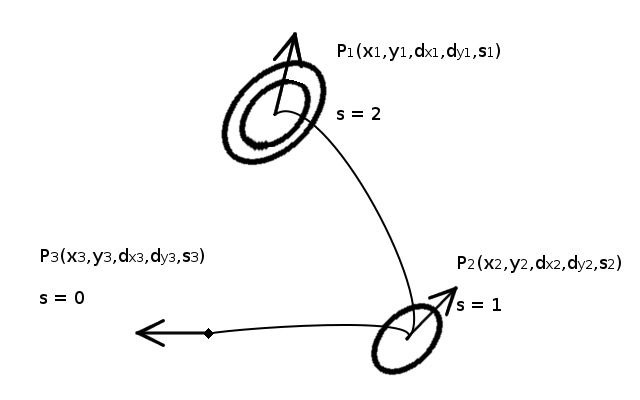
\includegraphics[scale=0.5]{images/proc_draw2}
\end{center}
\item Pontonkénti színszámítás: A képernyőt fellehet fogni mint egy n*m méretű mátix (képernyő szélessége: n, magassága: m). Az algoritmus pixelről pixelre haladva meghatározza annak értéket (0-255). A felbontás növekedés teljesítmény romláshoz vezet.
\end{enumerate}

A három karakter kirajzolás közül a procedurális rajzolás a legeffektívebb.

\subsection{Görbék}
\textit{Ide jöhet a Hermit}

\subsection{Karakter zajosítás}
\begin{itemize}
\item Pontszerű zajok

Tételezzük fel hogy a karakterünk mátrixa $M$ és zaj mátrixunk $N$ van. A két mátrix sor és oszlop száma megegyezik.

\begin{center}
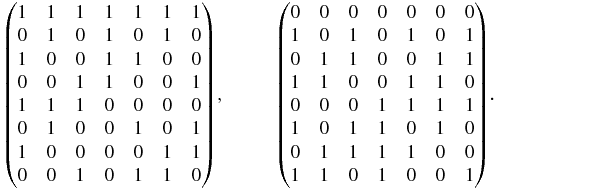
\includegraphics[scale=0.6]{images/noise_matrix}
\end{center}

M $\oplus$ N (a bináris operátor $\oplus$ később kerül meghatározásra). Fizikailag a zaj helytelen nyomtatási folyamatot jelent, vagy olyan helyzetet, amikor a felismerési rendszerben lévő gépi zaj torzítja a mintát. Feltételezzük továbbá, hogy minden egyes cellához tartozik zaj.
Ha egy adott cella (i, j) zajszintje nagyobb, mint az "1" vagy "fekete", akkor "1"-re kvantálódik. Más szavakkal, minden cella végül "1" vagy "0" besorolásnak kell alávetni. Megállapíthatjuk tehát, hogy a fent említett bináris művelet a következőket jelenti: 0 $\oplus$ 0 = 0,0 $\oplus$ 1 = 1, 1 ~ 0 = 1, és 1 $\oplus$ 1 = 1.
A zaj mátrix elemeinek megválasztásával különböző pontszerű zajokat tudunk létrehozni.
\item Elmosódások

Az elmosódás, amit símitásnak is neveznek, egyszerű és gyakran használt képfeldolgozási művelet. A simításnak sok oka van. A zaj növelése érdekében a elmosódás összpontosítunk.

Az elmosódás művelet végrehajtásához szűrőt alkalmazunk a képünkre. A szűrők legáltalánosabb típusa lineáris, amelyben a bemeneti pixelértékek (azaz $f(i+k, j+l)$) súlyozott összegével határozzák meg a kimeneti pixel értékét (azaz $g(i, j)$):

\[g (i, j) = \ sum_ {k, l} f (i + k, j + l) h (k, l)\]

$h(k, l)$ a kernelnek nevezik, ami nem más, mint a szűrő együtthatói. Segít megjeleníteni egy szűrőt, mint a képen csúsztatható együtthatók ablakát.

Sokféle szűrő létezik, mint például: Normalizált szűrő, gauss szűrő, medián szűrő.

A normalizált szűrő a legegyszerűbb. Minden kimeneti pixel a kernel szomszédainak átlaga (mindegyik egyenlő súlyokkal jár)

A kernel az alábbi:

\[K = \dfrac{1}{K_{szélesség} \cdot K_{magasság}}
\begin{matrix}
    1 & 1 & 1 & ... & 1 \\
    1 & 1 & 1 & ... & 1 \\
    . &. &. & ... & 1 \\
    . &. &. & ... & 1 \\
    1 & 1 & 1 & ... & 1   
\end{matrix}
\]
\item Forgatás
Forgatás
Egy kép elforgatását a szög $\theta$ értéket az alak átalakító mátrixával érjük el

$$M = \begin{bmatrix} cos\theta & -sin\theta \\ sin\theta & cos\theta   \end{bmatrix}$$

Az OpenCV azonban skálázható elforgatással rendelkezik, állítható forgó centrummal, így tetszőleges helyre forgatható. A módosított transzformációs mátrixot a

$$\begin{bmatrix}
\alpha &  \beta & (1- \alpha )  \cdot center.x -  \beta \cdot center.y \\ - \beta &  \alpha &  \beta \cdot center.x + (1- \alpha )  \cdot center.y
\end{bmatrix}$$

ahol:

$$\begin{array}{l}
\alpha =  scale \cdot \cos \theta , \\ \beta =  scale \cdot \sin \theta
\end{array}$$

Ennek az átalakulási mátrixnak a megtalálásához az OpenCV egy getRotationMatrix2D függvényt biztosít.

\begin{lstlisting}[language=Python]
img = cv2.imread('messi5.jpg',0)
rows,cols = img.shape

M = cv2.getRotationMatrix2D((cols/2,rows/2),90,1)
dst = cv2.warpAffine(img,M,(cols,rows))
\end{lstlisting}

\item Vágás
\item Takarás
\end{itemize}

\textit{Line break}\\\\

\begin{itemize}
\item Ecset dinamika
	\begin{itemize}
	\item \(P_1 = (x_1, y_1, d_{x_1}, d_{y_1}, s_1)\) \(P_2 = (x_2, y_2, d_{x_2}, d_{y_2}, s_2)\)
	\item Ecset szín (átmenetesség)
	\end{itemize}
\item Karakter kirajzolás
	\begin{itemize}
	\item Poligonos közelítés
	\item Procedurális rajzolás
	\item Pontonkénti színszámítás (fekete-szürke árnyalat-fehér)
	\item \textit{Görbék kirajzolása (Hermit)}
	\end{itemize}
\item Ideális karakter megjelenítés
\item Ideális karakter zajosítássa
	\begin{itemize}
	\item Különböző zajok
	\item Hálózat robosztussága
	\end{itemize}
\end{itemize}

\begin{comment}{Dolgozok a Hermit-es részen.}
\end{comment}

\begin{comment}{Ezek így vázlatnak jók, viszont az egyes pontokból legalább külön-külön szakaszoknak kellene majd lenni!}
\end{comment}
